\documentclass[12pt]{article}

\usepackage[margin=0.8 in]{geometry}
\usepackage{amsmath}
\usepackage{amssymb}
\usepackage{macros}
\usepackage{mathtools}
\usepackage{enumerate}
\usepackage{verbatim}
\usepackage{amsthm}

\title{}
%\content{}



\let \proj \undefined
\renewcommand{\tr}{ \mathrm{tr}}
\DeclareMathOperator{\SU}{SU}
\DeclareMathOperator{\proj}{proj}
\newcommand{\sS}{\mathscr{S}}
\DeclareMathOperator{\comp}{comp}
\newcommand{\A}{\mathcal{A}}
\renewcommand{\D}{\mathcal{D}}
\renewcommand{\e}{\epsilon}
\newcommand{\Are}{\A_{r,\e}}
\newcommand{\Kre}{K_{r,\e}}
\newcommand{\Dre}{\D_{r,\e}}
\newcommand{\rt}{\tilde{r}}
\newcommand{\et}{\tilde{\e}}
\newtheorem{definition}{Definition}
\newenvironment{solution}
  {\begin{proof}[Solution]}
  {\end{proof}}
\newtheorem{example}{Example}
\newtheorem{exercise}{Exercise}

\newcommand{\vr}{\mathbf{r}}
\newcommand{\vF}{\mathbf{F}}

\newtheorem{theorem}{Theorem}



\begin{document}
\section*{Change of variables}
What to know
\begin{enumerate}
\item Be able to find the image of a transformation
\item Be able to invert a transformation
\item Be able to find the Jacobian of a transformation
\item Be able to set up and solve an integral using a change of variables.
\item Might be useful to remember the transformation formula for rotations.
\end{enumerate}

\subsubsection*{Motivation}
In calculus 2 we saw a way of changing the variable in an integral, that is, \begin{equation}\label{eq1}\int_a^b f(x) dx = \int_c^d f(g(u))g'(u)du,\end{equation} where $c= g^{-1}(a) $ and $d= g^{-1}(b)$ and this helped simplify the calculations. We will now see how to generalize this method to double integrals.
\vspace{.1 in}


Let's see a familiar example. 
\begin{example} A half annulus $D=\{(x,y):1\leq x^2+y^2\leq 4, y\geq 0\}$ is more complicated to describe in Cartesian coordinates, but easier in polar: $$D=\{(r,\theta):1\leq r\leq 2, 0\leq \theta \leq \pi\}.$$ If we draw it on the $r-\theta$ plane we'll notice it looks like a rectangle.
\end{example}


\begin{figure}
\centering
\parbox{5cm}{
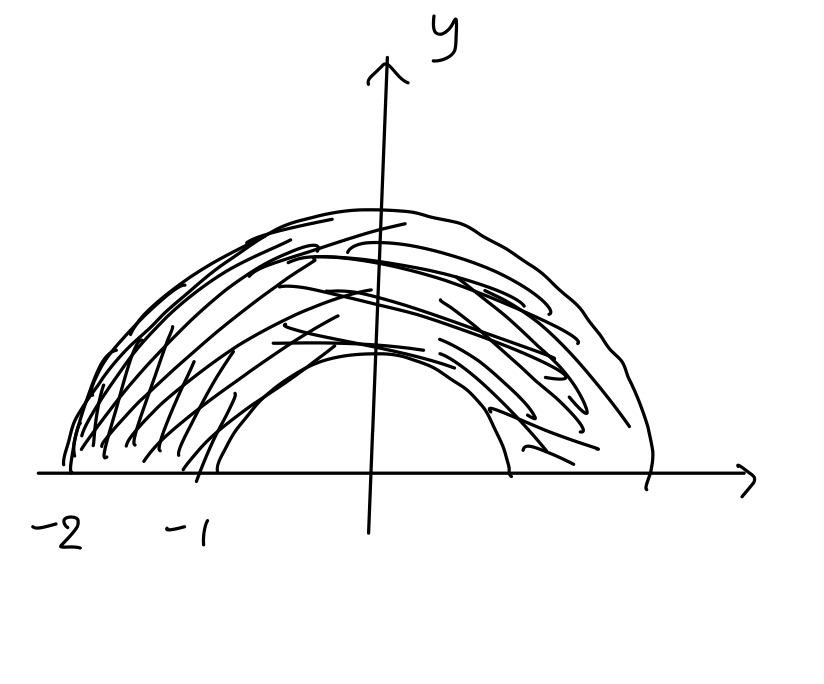
\includegraphics[width=5cm]{annulus.jpeg}
\caption{A half annulus on the $xy$ plane}}
%\label{}
\qquad
\begin{minipage}{5cm}
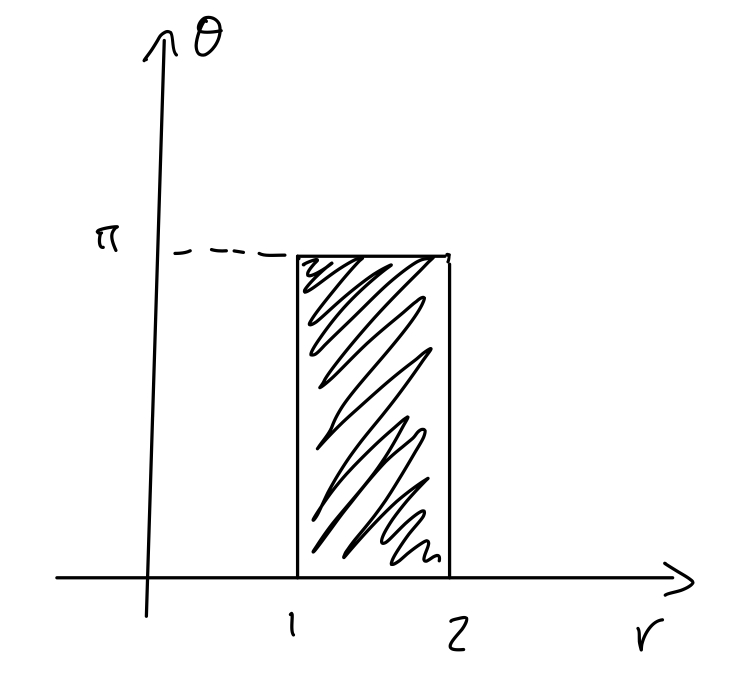
\includegraphics[width=5cm]{rectangle.jpeg}
\caption{The corresponding rectangle on the $r\theta$ plane}
%\label{fig:2figsB}
\end{minipage}
\end{figure}



\vspace{.1 in}
Goal of today's section is to simplify the evaluation of \begin{equation}\label{eq2}\iint_R e^{xy}\ln(\frac{y}{x})dx dy,\end{equation} where $R$ is bounded by \begin{align*}
&y=\frac{1}{x}, & y=\frac{4}{x}, &&y=x, && y=4x,
\end{align*} in the first quadrant.

\vspace{.1 in}
\subsubsection*{Transformations}
Similarly to \eqref{eq1} we'll need a function $T$ from a subset of the $uv$ plane to a subset of the $xy$ plane. We will call such a function \textbf{transformation} and write $$T(u,v)=(x,y),$$ or $$\begin{cases} x=x(u,v)\\
y=y(u,v)
\end{cases}
$$ (that is, $x$ and $y$ are written as functions of $u, v$).

We will assume that $x$ and $y$ have continuous partial derivatives with respect to $u$ and $v$. Such a transformation is called $C^1$.

The \textbf{{domain}} of $T$ is the subset of $\R^2$ plane where it's defined. The \textbf{image} $R$ of a subset $S$ of the domain under $T$ is the output we obtain once we feed $T$ with all points of $S$ and we write $R = T(S)$. 

\subsubsection*{Inverse transformation}


For integration, we will need to work with \textbf{invertible} transformations. This means that we can solve for $ u, v$, that is, for each pair of $x, y$ find a unique pair of $u, v$ such that $(x,y)=T(u,v)$. This gives another transformation, called the \textbf{inverse transformation},
$$\begin{cases} u=u(x,y)\\
v=v(x,y)
\end{cases},
$$ 
which we will denote by $T^{-1}$. Then the domain-image relation can be written in terms of $T^{-1}$ as $S=T^{-1}(R)$. Finally, we'll need $T^{-1}$ to be $C^1$ as well. If $T$ is invertible, then $T^{-1}$ is invertible too, and its inverse is $T$ itself.

\begin{example}\label{exmpl} A transformation that is \textbf{not} invertible is $$\begin{cases}x&=u^2\\
y&=v
\end{cases}$$ on $\R^2$. Trying to solve for $(u, v)$, you'll have to make a choice of roots, so you can't solve uniquely! 
\end{example}




%\textbf{Tip:} The easiest way to find the image of a transformation is to find the image of its boundary curves. 

\vspace{.1 in}

\subsubsection*{Jacobian Determinant.}
In the Change of Variables in one variable he had a derivative show up, so we'll make sense of a derivative of a transformation, and give an easy criterion to check the two $C^1$ conditions mentioned above (one for $T$ and one for $T^{-1}$). This will be done via the Jacobian Determinant. 

If $x=x(u,v)$, $y=y(u,v)$ is a $C^1$ transformation, the Jacobian determinant is given by 
$$\frac{\p (x,y)}{\p (u,v)}:=\left|
\begin{array}{cc}
 \frac{\p x}{\p u} & \frac{\p x}{\p v} \\
 \frac{\p y}{\p u} & \frac{\p y}{\p v} \\
\end{array}
\right| =  \frac{\p x}{\p u}\frac{\p y}{\p v} -\frac{\p x}{\p v}\frac{\p y}{\p u}.$$



\textbf{Remark:} The notation above (which is the one used by the book) is probably not the most standard one in literature. You may also see it often denoted by $|JT(u,v)|$ or $|DT(u,v)|$.

Regarding the $C^1$ conditions, there is this theorem:
\begin{theorem}
If a $C^1$ transformation is invertible on its domain and the Jacobian determinant is always non-zero on the domain, then the inverse transformation is $C^1$.
\end{theorem}




\textbf{In practice:} If nothing too horrible happens to the partial derivatives involved in the Jacobian determinant (such as go to $\infty$ somewhere in the domain) and the Jacobian doesn't vanish in the domain then both $C^1$ conditions are satisfied.

\textbf{Remark:} Looking at the transformation in Example \eqref{exmpl} you'll see that its Jacobian determinant vanishes on the $v$ axis, so that's another reason we wouldn't like it for integration purposes.


\subsubsection*{Integration}

Finally, the theorem we wanted to get to:
\begin{theorem} \label{thm}{(Change of variables)} For a $C^1$ invertible transformation $T$ with $C^1$ inverse, if $T$ is written as $x=x(u,v)$ and $y=y(u,v)$, we have 
$$\iint_R f(x,y) dA =\iint_S f(x(u,v),y(u,v))\big|\frac{\p (x,y)}{\p({u},{v})} \big|du dv,$$ where $ S=T^{-1}(R)$.
\end{theorem}

\textbf{Remarks:}
The Jacobian determinant in the integration formula above has an absolute value around it, which is not the case for the definition: So, if you're just asked to write the Jacobian determinant it might be positive or negative.

 
\subsection*{Some strategies on solving problems}

If the transformation is not given, we have to figure it out based on the domain and/or the formula of the function (usually the domain). Looking at our goal of the day integral, for example, we observe that the boundary curves are $y=\frac{1}{x},  y=\frac{4}{x}, y=x,$ and $ y=4x$.

We look for patterns, that is, expressions of $x$ and $y$ that repeat themselves. Here, we see that $xy$ and $\frac{y}{x}$ repeat themselves, so it makes sense to set $$u=xy$$ and $$v=\frac{y}{x}$$ (In the previous notation this is $T^{-1}$). This will make the domain easily expressible in terms of $u$, $v$.

\subsubsection*{Summarizing the steps}
Once we have to calculate an integral over a domain $R$in the $xy$ plane using a transformation:
\begin{enumerate}
\item If a transformation $x=x(u,v)$, $y=y(u,v)$ is not given, try to figure it out from the equations.
\item For this class, I will usually tell you that the transformation is invertible. If this is not known to you, solve for $u$, $v$ to make sure.
\item Find $T^{-1}(R)$, which will be a subset of the $uv$ plane. To do this, it's usually enough to plug in $x=x(u,v)$ and $y=y(u,v)$ in the equations describing the boundary of $R$ and see what the resulting curves look like.
\item Find the Jacobian determinant, making sure that the partial derivatives involved don't behave badly, and check that it is non-zero on $T^{-1}(R)$.
\item Apply the formula in Theorem \ref{thm} to integrate.
\end{enumerate}




\subsection*{Solve the integral of \eqref{eq2}}
We find the image $S=T^{-1}(R)$. Look at bounding curves: $$y=\frac{1}{x}\implies xy=1\implies u=1$$
$$y=\frac{4}{x}\implies xy=4\implies u=4$$
$$y=x\implies \frac{y}{x}=1\implies v=1$$
$$y=4x\implies \frac{y}{x}=4\implies v=4$$
So $S$ is a square in the $uv$ plane, which is really easy to integrate over!

To continue, we need to write $x$ and $y$ in terms of $u$, $v$, that is, solve for $x $ and $y$:
$$\begin{cases}
u=xy\\
v=\frac{y}{x}
\end{cases}\implies 
\begin{cases}
uv=y^2\\
\frac{u}{v}=x^2
\end{cases}
\implies
\begin{cases}
y=\sqrt{uv}\\
x=\sqrt{\frac{u}{v}}
\end{cases}.
$$


Find the Jacobian determinant:

$$\frac{\p (x,y)}{\p (u,v)}=\left|
\begin{array}{cc}
 \frac{1}{2\sqrt{uv}} & \frac{-\sqrt{u}}{2v^{3/2}} \\
 {\frac{\sqrt{v}}{2\sqrt{u}}} & \frac{\sqrt{u}}{2\sqrt{v}} \\
\end{array}
\right| = \frac{1}{2v}\neq 0$$


Applying our theorem, $$\iint_R e^{xy}\ln(\frac{y}{x})dxdy=\iint_S e^u \ln(v)|\frac{1}{2v}|dudv=\int_1^4\int_1^4 e^u \ln(v)\frac{1}{2v}dudv=(e^4-e)(\ln2)^2.$$

\subsection*{A useful class of transformations}
 In general, a transformation need not carry straight lines to straight lines, as we saw before. However, there is a special type of transformations that do. They are called \textbf{affine transfromations} and they are of the form \begin{align*}
 u & = a_{11}x+a_{12}y+b_1\\
 v & = a_{21}x+a_{22}y+b_2
 \end{align*}
In matrix notation, you can write this as $$\left(\begin{array}{c}
u \\ 
v
\end{array}\right)=\left(\begin{matrix}
a_{11} & a_{12} \\ 
a_{21} & a_{22}
\end{matrix}\right)\left(\begin{array}{c}
x \\ 
y
\end{array}\right)+\left(\begin{array}{c}
b_1 \\ 
b_2
\end{array}\right) . $$
If $b_1$=$b_2$=0, then the transformation is called \textbf{linear} and it sends lines through the origin to lines through the origin. Affine transformations are useful because given a domain that is bounded by straight lines we can find its image under the transformation by finding the image of the points of intersection between the lines and connecting them by straight lines.

A particular type of of linear transformations are the \textbf{orthogonal transformations}, that in addition preserve lengths and angles.

Such are the \textbf{rotations} by angle $\theta$:
 \begin{align*}
 u & = \cos(\theta)x-\sin(\theta)y\\
 v & = \sin(\theta)x+\cos(\theta)y.
 \end{align*}
Also the reflection about the $y$ axis:
 \begin{align*}
 u & = -x\\
 v & = y.
 \end{align*}
\begin{exercise} What transformation would you use to integrate more easily over a domain that looks like that in Figure \ref{fig1}?
\begin{figure}
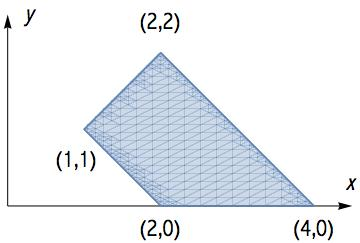
\includegraphics[scale=.3]{problem5C.jpg}
\caption{A domain.}
\label{fig1}
\end{figure}
\end{exercise}


\end{document}

